As explained previously, the low di-jet invariant mass and low jet rapidity separation is dominated by tri-bosons production.
Therefore a comparison of the various approximation in an \emph{inclusive} phase-space volume.
To that end, we have chosen for the inclusive fiducial volume to take the following values for the VBS cuts 

\begin{equation}
\label{eq:inclusive}
	m_{jj} > 200\GeV\,,\qquad |\Delta y_{jj}| > 2 .
\end{equation}


The figure is Fig.~\ref{fig:ratio2d_LO}, the ratio of double-differential cross sections in the plan $\left(m_{\Pj\Pj}, \Delta y_{\Pj\Pj}\right)$ is shown.
Two plots are displayed: the ratio of the $|t|^2 + |u|^2$ and $|s|^2 + |t|^2 + |u|^2$ approximations over the full calculation, respectively.
In the first case, the approximation is good within $\pm10\%$ over the whole range apart in the low invariant-mass region at both low and large rapidity difference.
The low rapidity difference region possesses remnants of the tri-bosons contributions.
It is therefore expected that the $|t|^2 + |u|^2$ approximations fails in this region.
The second plot, where the $|s|^2 + |t|^2 + |u|^2$ approximation is considered, displays a better behaviour in the previously mentioned region.
The full calculation is approximated at the level of $\pm10\%$ everywhere apart in the upper left corner where the inclusion of $s$-channel contributions did not improve the approximation.
This is due to ...

\begin{figure}[hbt]
\centering
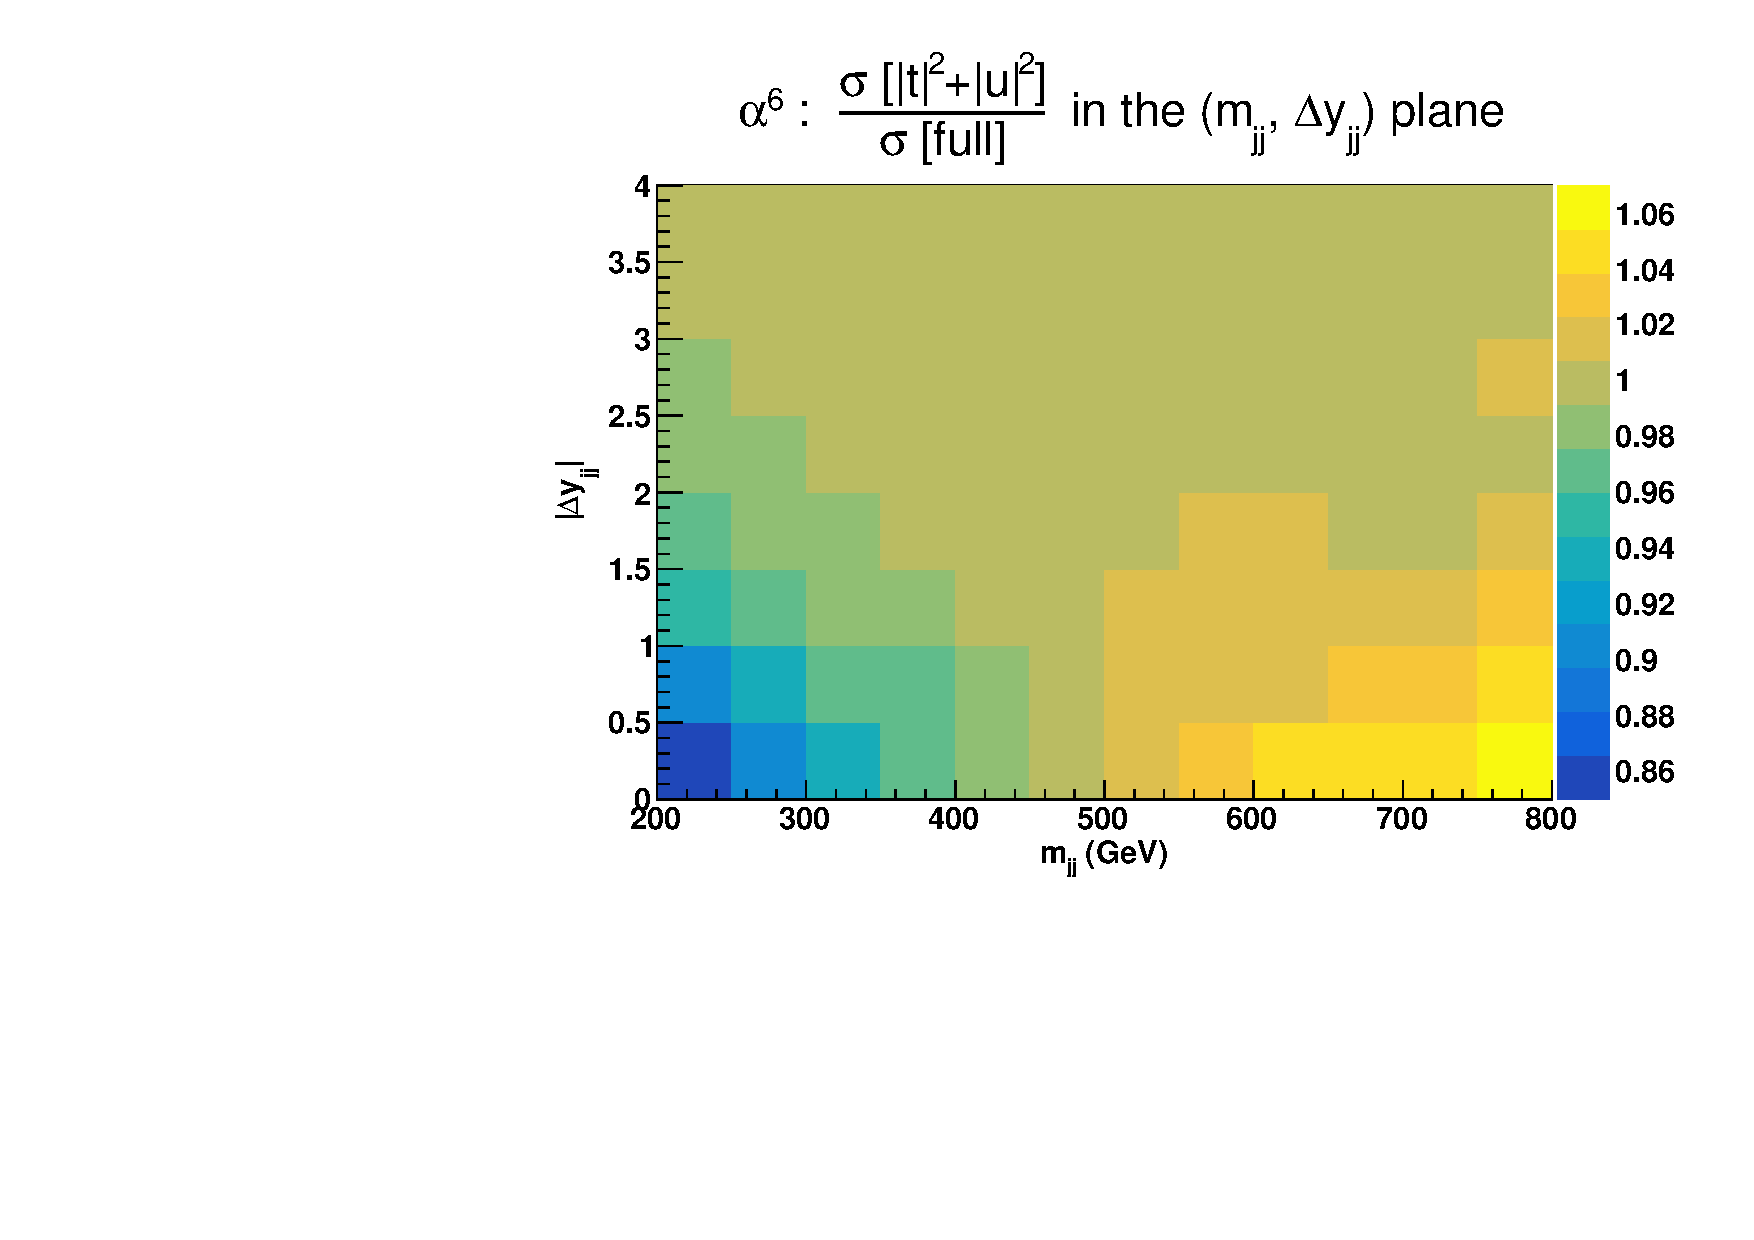
\includegraphics[scale=0.395]{figures/scanfigures/ratio_tu.pdf}
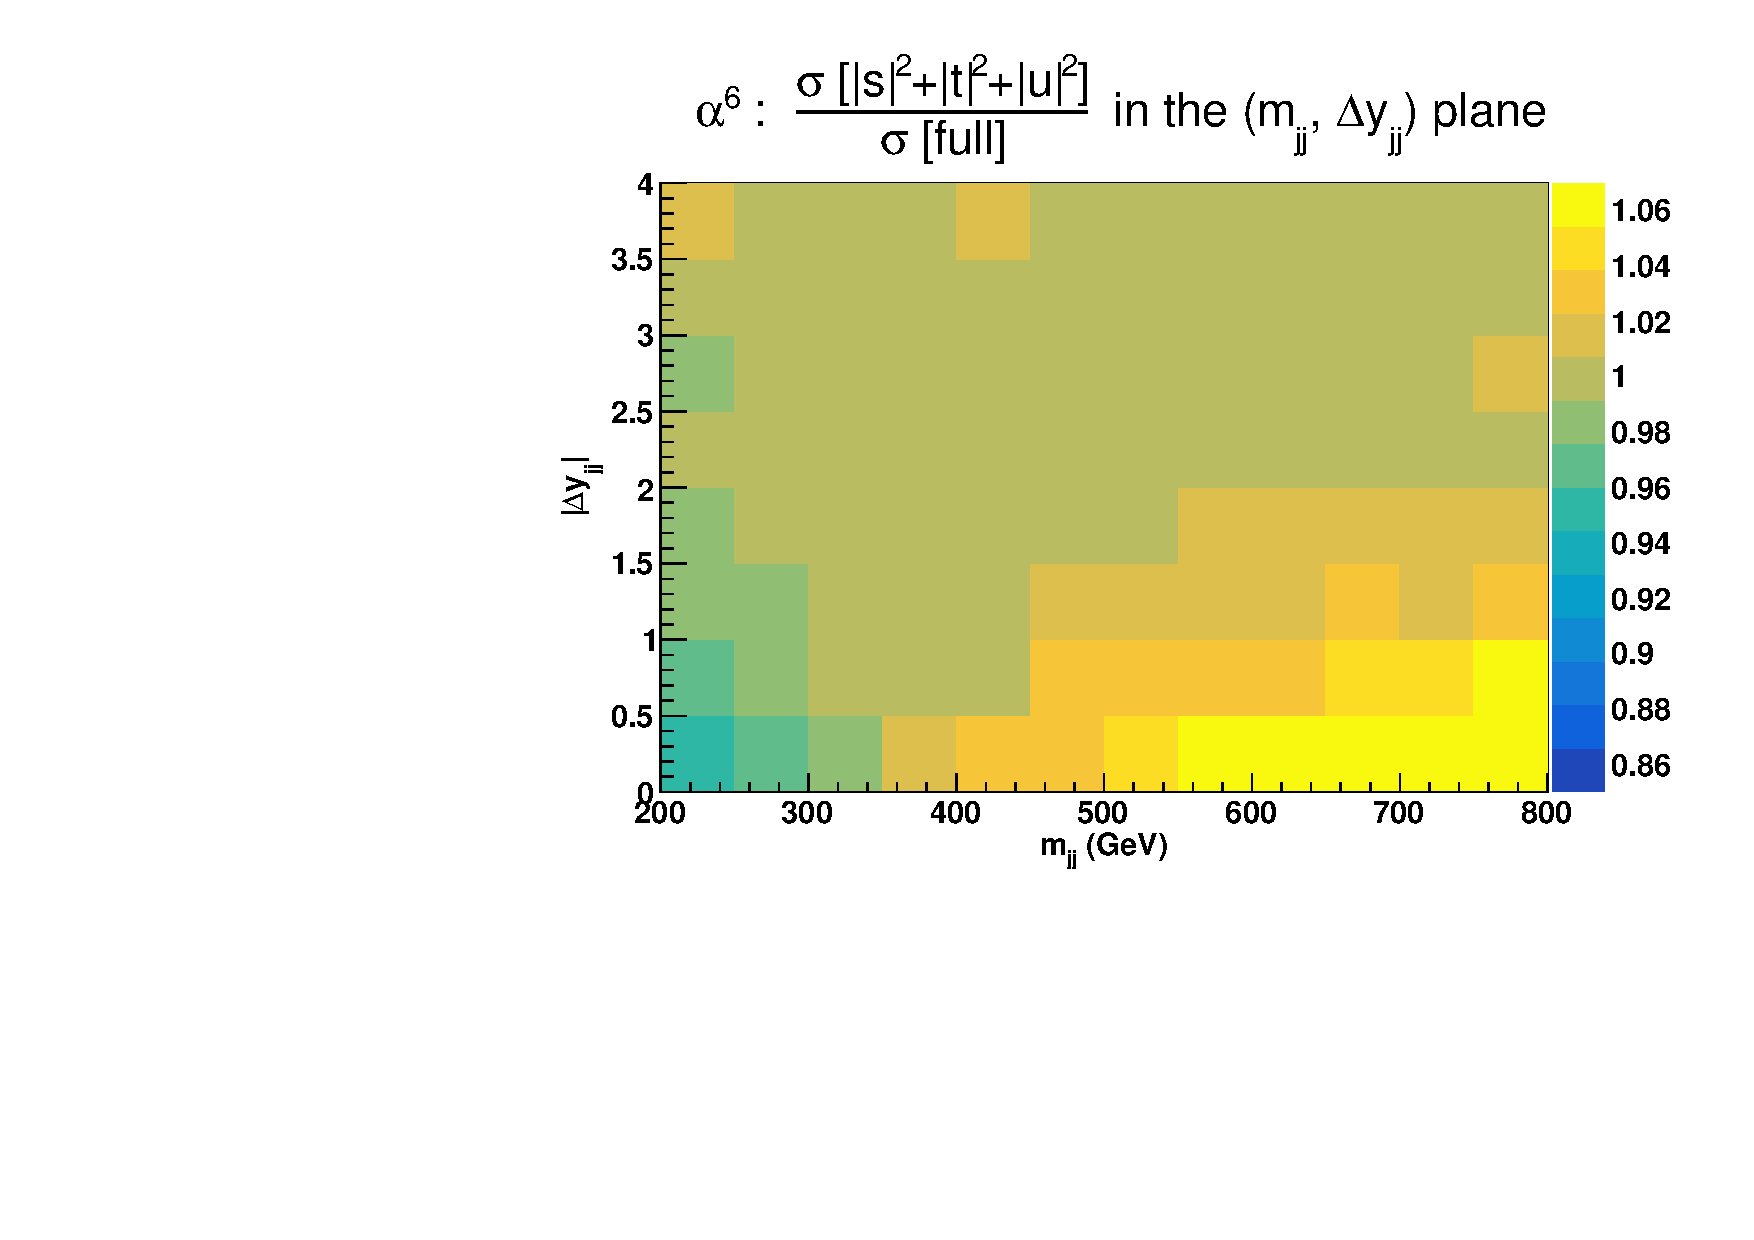
\includegraphics[scale=0.395]{figures/scanfigures/ratio_stu.pdf}
\caption{Cross sections (fb) per bin in the plan $\left(m_{\Pj\Pj}, \Delta y_{\Pj\Pj}\right)$ at order $\mathcal{O}(\alpha^6)$. 
Ratio of approximated squared amplitudes over the full matrix element. The approximated squared amplitudes are computed as $|\mathcal{A}|^2 \sim |t|^2 + |u|^2$ (left) and $|\mathcal{A}|^2 \sim |s|^2 + |t|^2 + |u|^2$ (right).}
\label{fig:ratio2d_LO}
\end{figure}

